\documentclass[letterpaper,10pt]{article}
\usepackage{hyperref}
\usepackage[scriptsize,bf]{caption}
\usepackage{fullpage}
\usepackage{textcomp}
\usepackage{times}
\usepackage{cite}
\usepackage{fancyvrb}
\usepackage{moreverb}
\usepackage{graphicx}
\usepackage{multicol}

\makeatletter
\newenvironment{figurehere}
{\def\@captype{figure}}
{}
\makeatother

\newcommand{\squishlist}{\begin{list}{$\bullet$}
  {\setlength{\itemsep}{0pt}
    \setlength{\parsep}{3pt}
    \setlength{\topsep}{3pt}
    \setlength{\partopsep}{0pt}
    \setlength{\leftmargin}{1.5em}
    \setlength{\labelwidth}{1em}
    \setlength{\labelsep}{0.5em}
  } }

\newcommand{\squishend}{\end{list}}

\title{LRUMAP: $O(1)$ LRU for Classifying Network Probes}
\author{Nick Black and Jolene Tarosky\\
CS7260 Project, Spring 2010}
\date{}

\begin{document}
\maketitle

\begin{abstract}
Network administrators, particularly in proactively secure environments such
as military installations, banks and SCADA sites, seek to discriminate standard
network accesses from reconnaissance. In both host-based intrusion prevention
systems (such as Solar Designer's \texttt{scanlogd}\footnote{\url{http://www.openwall.com/scanlogd/}})
and network-level applications (such as the open source Snort\footnote{\url{http://www.snort.org/}} IDS),
this is accomplished via comparing against some threshold the ratio of a remote
host's successful accesses of the network to unsuccessful accesses. While a
successful access will almost inevitably elicit some response packet, a
reconnaissance may well receive no reply. Classification ought thus not be performed
at reply time, but only upon a potential probe's ingress.

First-packet classification requires predicting the success of a network access.
Especially among environments heterogeneous in ownership or architecture (data centers, research facilities,
development firms, etc), the likelihood of a given service (identified by host
and transport addresses, and network protocol) existing can vary widely from
host to host. Tracking these services dynamically is a natural fit for LRU, but
traditional $O(N)$ or even $O(lgN)$ LRU implementations are too slow for
backbone routers and IPS devices. We introduce LRUSET, a $O(1)$ true LRU scheme
which becomes more space-efficient as the number of monitored hosts increases.
We then illustrate several other counting problems from networking algorithmics
which could be benefited by this novel data structure.
\end{abstract}

\begin{multicols}{2}
\section{Introduction}

\section{LRUMAP Data Structure}
\section{LRUMAP Algorithms}
\section{Beyond LRUMAP}
\subsection{Extensions}
It is trivial to adapt LRUMAP to the Most-Recently-Used methodology, employed
by page caches when a ``looping sequential''\cite{dewitt} access pattern is
detected.
\subsection{Optimizations}
It may not be necessary to perform true, precise LRU. Many systems, including
the cache controllers of Intel\cite{shanley} and Via processors, make use of
approximation schemes such as \textit{pseudo-LRU}.
\begin{figurehere}
	\centering
	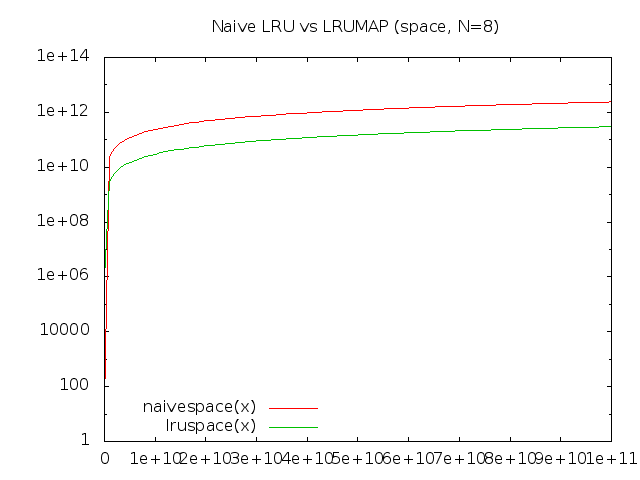
\includegraphics[width=\columnwidth]{out/lrumap8.pdf}
	%\caption{Eighth-order LRU}
\end{figurehere}
\begin{figurehere}
	\centering
	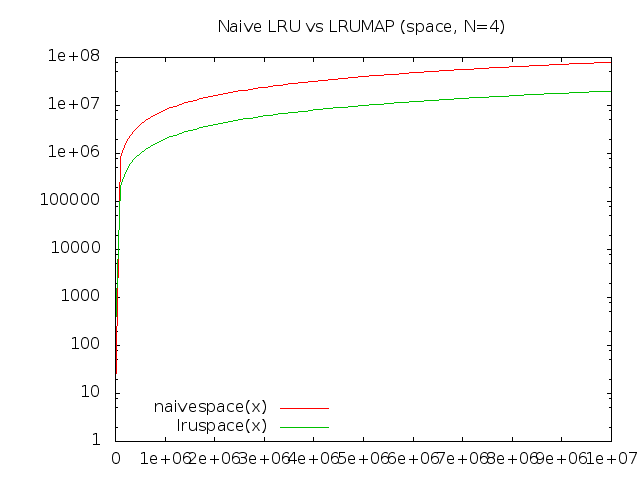
\includegraphics[width=\columnwidth]{out/lrumap4.pdf}
	%\caption{Fourth-order LRU}
\end{figurehere}

\cite{varghese}
\cite{xu}
\bibliographystyle{acm}
\bibliography{cs7260final}
\end{multicols}
\end{document}
